% =============================================================================
% UFFIZI RL: TECHNICAL PROJECT PAPER
% Build from this directory with: pdflatex uffizi_paper.tex
% =============================================================================
\documentclass[11pt]{article}

\usepackage[a4paper,margin=2.25cm]{geometry}
\usepackage[T1]{fontenc}
\usepackage{fourier}
\usepackage{microtype}
\usepackage{amsmath,amssymb,mathtools}
\usepackage{booktabs}
\usepackage{graphicx}
\usepackage{tabularx}
\usepackage{xcolor}
\usepackage{float}
\usepackage[hidelinks]{hyperref}

\graphicspath{{../outputs/figures/}}

\setlength{\parindent}{1.15em}
\setlength{\parskip}{0.25em}
\renewcommand{\arraystretch}{1.18}

\newcommand{\R}{\mathbb{R}}
\newcommand{\E}{\mathbb{E}}
\newcommand{\Acal}{\mathcal{A}}
\newcommand{\ind}{\mathbb{1}}
\newcommand{\added}[1]{{\color{green!50!black}#1}}
\newenvironment{addedblock}{\begingroup\color{green!50!black}}{\endgroup}
\newcommand{\fig}[1]{../outputs/figures/#1}
\newcolumntype{Y}{>{\raggedright\arraybackslash}X}
\newcolumntype{P}[1]{>{\raggedright\arraybackslash}p{#1}}

\title{\textbf{The Art of Queueing}\\
\large Reinforcement Learning for visitor flow at the Gallerie degli Uffizi in Florence}
\author{Marco Canal \and Michael Duarte Gon\c{c}alves \and Mircea-Adrian Guinea}
\date{Reinforcement Learning \\ June 2026}

\begin{document}
\maketitle

\begin{abstract}
The Uffizi Gallery makes congestion visible as a reinforcement-learning problem: capacity is not
scarce everywhere, but demand concentrates around Botticelli, Leonardo, Raphael-Michelangelo and
Caravaggio. We use two linked model layers. A minute-step agent-based simulator moves
heterogeneous visitors through the room graph and evaluates institutional interventions under a
revenue-preservation constraint. On top of those simulated crowds, RL agents solve the
visitor problem: when to stay, when to move and how far ahead, under RAMA
\added{(Reservation-Anchored Masterpiece Access, a booking layer for fixed 10-minute masterpiece
windows)}, to reserve masterpiece slots. The technical work is mostly formulation. Appreciation
progress makes dwell decisions Markovian; dense closing pressure prevents late trapping; reward design
discounts congestion without making masterpieces unattractive; action masks keep PPO on legal graph
and booking-phase choices. In the final simulator evaluation, the all-11 bundle \added{(the full
intervention scenario combining the active museum policy switches)} raises completed welfare by 31\%
at 5,000 visitors with revenue essentially preserved. Five-seed MaskablePPO booking policies beat
matched no-booking baselines across profiles and crowds in every cell.
\end{abstract}

\section{Problem and Modeling Strategy}

The project starts from a common-pool resource problem. The Uffizi has enough total floor area to
serve many visitors, but visitor utility is degraded when a large share of demand arrives in the same
rooms at the same time. The clearest bottleneck is the Botticelli chain: rooms A11 and A12 lie on a
forced path and contain \emph{Primavera} and \emph{The Birth of Venus}. Leonardo and
Raphael/Michelangelo generate secondary peaks, while many other galleries remain underused. The RL
question is whether a learner can use time, route choice and reservation lead time to obtain a better
visit than a fixed itinerary.

\added{The implementation has two streams.} At the museum-wide level, a minute-step simulator runs a
full day of heterogeneous visitors under the legal 900-person capacity constraint. Interventions alter
arrival curves, access rules, prices and secondary attractions; \added{they pass the director gate only if
they improve welfare without making revenue politically infeasible.} At the individual level, one
\added{booking agent} optimizes a visit conditional on either the status-quo or intervened crowd process. In
the status quo, the relevant action is mostly whether to remain in a room or continue along a planned
route. Under RAMA, the main action happens before entry: the visitor chooses how far in advance
to reserve masterpiece slots and must then pace the walk to reach those windows.

Keeping the streams separate avoids mixing two outputs. The simulator produces the museum-wide
welfare and revenue statistics. The RL agents estimate an optimized individual visit under a fixed
population process, so a single-visitor policy is not by itself an evaluation of the institutional
intervention.

\added{Our contribution is threefold: (i) we formulate the Uffizi visit as linked population and
individual RL problems; (ii) we build a RAMA booking MDP with reservation lead time as an action; and
(iii) we document the environment changes that made learning work: action masking, appreciation
progress in the observation and dense rewards for closing time and bad bookings.}

\section{The virtual Uffizi}

\subsection{Graph and calibration}

The physical museum is encoded as a directed graph $G=(V,E)$ built from the 98 rooms emphasized in the
slides plus operational nodes such as the entry, staircases, terrace and exit. Each room carries four
central attributes: cultural importance, dwell-time magnetism, legal or effective capacity and
section. Ordinary doors are represented bidirectionally; staircases and exit routes are directed. The topology is validated with structural invariants:
weak connectivity, reachability from the entry, reachability of an exit from every gallery, high
degree for the main corridor hubs and a forced Botticelli chain A10--A11--A12--A13.

Visitors arrive through 37 fifteen-minute entry slots with a broad morning-weighted envelope. The
simulator uses a one-minute time step, a 615-minute baseline day (08:15--18:30) and a final-entry
cutoff at 17:30. The full intervention scenario extends the day to 720 minutes. The population mix is
60\% Instagram tourists, 30\% normal tourists and 10\% art lovers. Instagram tourists concentrate on
famous rooms and the panoramic terrace, move quickly and are nearly crowd-indifferent. Normal
tourists visit the famous rooms plus a few canonical additions, such as the Tribune and Caravaggio.
Art lovers have heterogeneous taste vectors, longer dwell times, stronger crowd aversion and a higher
probability of accepting alternative routes.

The movement model is local and stochastic. Conditional on deciding to move, a visitor chooses among
neighbors with weights of the form
\[
w_{i\to j}=\max\{0.01,\; b_{\text{route}}(j)+b_{\text{importance}}(j)+b_{\text{crowd}}(j)\},
\qquad
P(i\to j)=\frac{w_{i\to j}}{\sum_{k\in N(i)} w_{i\to k}}.
\]
\added{Here $i$ is the current room, $j$ is a neighboring room, $N(i)$ is the set of legal next rooms,
and $P(i\to j)$ is the one-minute movement probability. The three $b$ terms are local pulls: route
following, room value and crowd avoidance. The $0.01$ floor prevents a legal doorway from becoming
impossible. A visitor in A11 therefore weighs the recommended Botticelli route against the appeal and
crowding of nearby rooms, then samples a next step rather than following a fixed script.} The executable simulator adds RAMA
slots, low-budget exit seeking, tour groups, Caravaggio priority and masterpiece bypasses. The
simulator is behavioral: it creates plausible crowd pressure, while the RL wrappers solve the
controlled visitor problem separately.

\subsection{Museum interventions}

The intervention catalog contains access controls, price instruments, time architecture and demand
redistribution. The slide language calls the final scenario ``all 11'' because the publication catalog
has eleven intervention specifications, including two pre-bundled combinations. The implementation
merges these specifications with last-write-wins semantics into nine distinct active switches: RAMA,
secondary-attractor enrichment, extended hours, dynamic pricing, resident annual pass expansion,
timed entry, quiet hours, a tour-group cap of 10 and a EUR150 group surcharge. A separate portfolio
optimizer screens interventions individually and then applies greedy forward selection followed by
one-step local search on a scalarized welfare/revenue objective. That optimization is an
economic sensitivity check, but the RL booking agents are trained in the all-11 world because it is the
environment in which RAMA access is active and internally consistent.
\begin{addedblock}
The institutional screening rule is
\[
\mathcal I^*\in\arg\max_{\mathcal I\in\Omega} W(\mathcal I)
\quad\text{s.t.}\quad R(\mathcal I)\ge (1-\delta)R(0),
\]
where $\mathcal I$ is an intervention bundle, $\Omega$ is the set of bundles we test, $W$ is simulated
completed welfare, $R$ is ticket revenue, $R(0)$ is status-quo revenue and $\delta$ is the allowed
revenue loss. The constraint rejects an intervention that improves the visit only by giving up too
much revenue.
\end{addedblock}

\begin{table}[t]
\centering
\caption{Museum-wide simulator results: status quo versus the all-11 intervention world. Welfare is
total completed visitor welfare. Revenue is daily ticket revenue in EUR.}
\label{tab:museum-wide}
\begin{tabular}{lrrrrr}
\toprule
Crowd & Welfare base & Welfare int. & Gain & Revenue base & Revenue int. \\
\midrule
500   & 277,256   & 343,507   & +24\% & 11,542 & 11,317 \\
2,500 & 1,106,175 & 1,274,045 & +15\% & 56,604 & 56,544 \\
5,000 & 1,514,458 & 1,986,425 & +31\% & 96,502 & 94,792 \\
\bottomrule
\end{tabular}
\end{table}

Figure~\ref{fig:density} gives the corresponding spatial evidence. At the 5,000-visitor crowd,
Botticelli peak density falls from 1.82 to 1.00 and traffic is distributed over a longer operating
window. The intervention does not make the museum empty; rather, it keeps the highest-demand rooms
closer to usable capacity.

\begin{figure}[t]
\centering
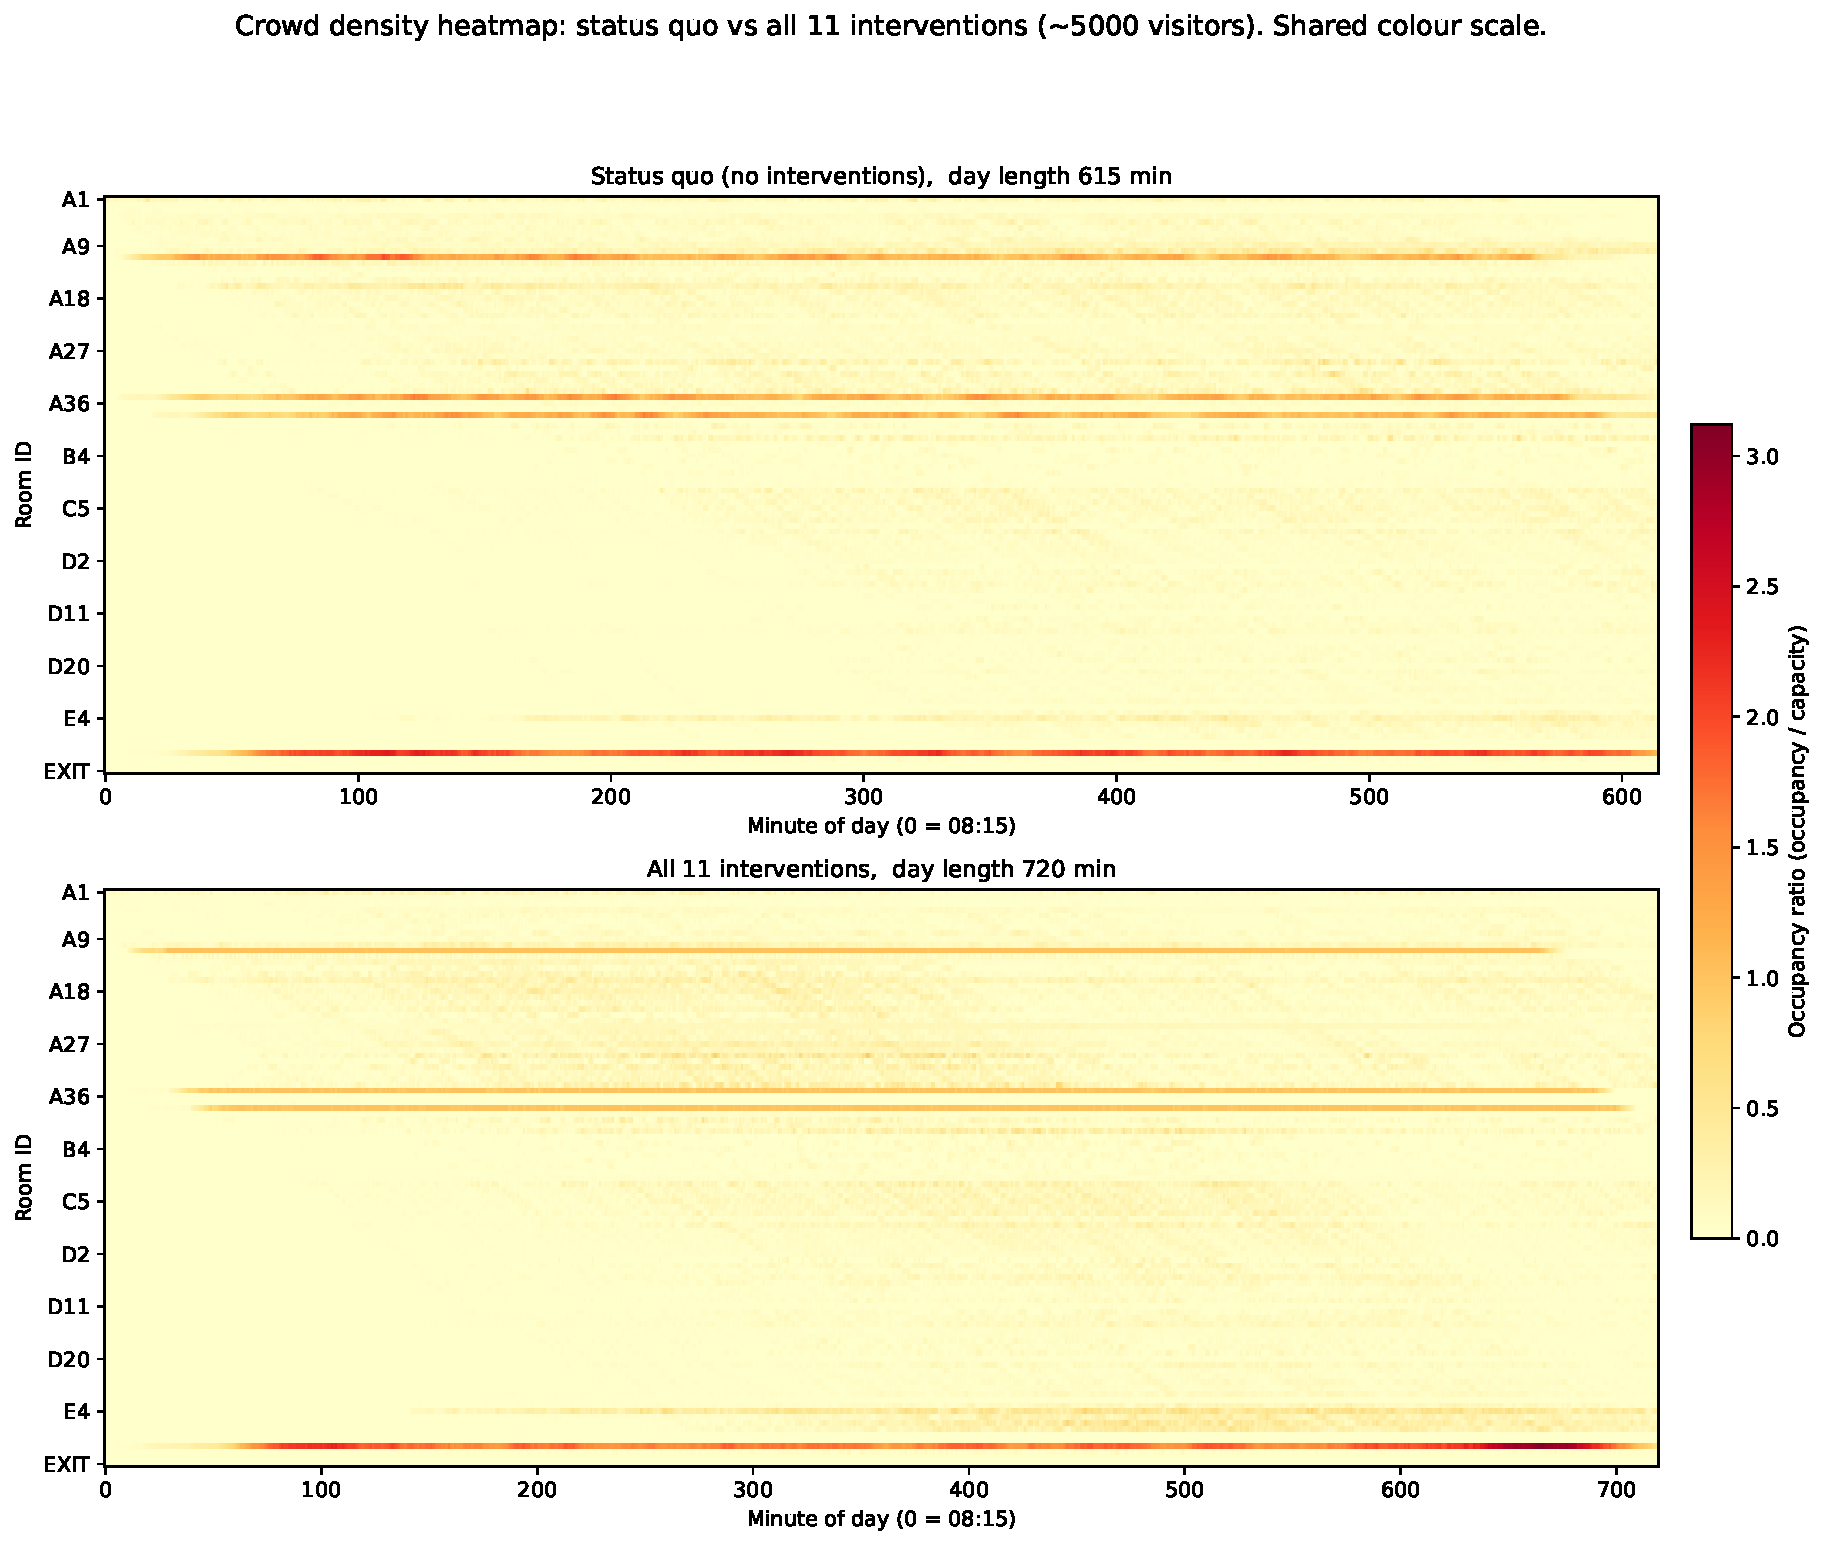
\includegraphics[width=\linewidth]{36_density_heatmap_intervened.pdf}
\caption{Crowd density under the status quo and under the full intervention bundle. The color scale is
shared, so cooling of the red bands corresponds to a real reduction in occupancy over capacity.}
\label{fig:density}
\end{figure}

\section{MDP Formulations}

Each individual agent is a discounted Markov decision process
$\mathcal{M}=(\mathcal{S},\mathcal{A},P,r,\gamma)$, but the relevant state and action space change
with the decision problem. Defining what the visitor observes and which actions are legal mattered at
least as much as choosing PPO or DQN.
\begin{addedblock}
For a visitor profile $p$, the generic objective is
\[
J(\pi)=\E_{\pi,P_p}\!\left[\sum_{t=0}^{T}\gamma^t r_p(S_t,A_t)\right].
\]
Here $\pi$ is the visitor policy, $P_p$ is the simulator transition rule for profile $p$, $T$ is the
visit horizon, $\gamma$ discounts later minutes and $r_p$ is the profile-specific reward. The objective
values the whole visit, so delayed events such as missed slots or a late exit still matter. The full
simulator state can be Markovian only when it includes room, clock, crowd tensor, reservations, visitor
history, appreciation progress and exit slack. The policy receives a compact observation
$o_t=\phi(S_t)$, so the implemented agents are engineered MDP approximations to a partially observed
visitor problem.
\end{addedblock}

\begin{table}[t]
\centering
\small
\caption{The three MDP families used in the project.}
\label{tab:mdps}
\begin{tabularx}{\linewidth}{@{}P{0.16\linewidth}Y P{0.20\linewidth}P{0.17\linewidth}@{}}
\toprule
Setting & State & Action & Algorithms \\
\midrule
Toy museum &
Discrete 5-tuple: room, time bin, Botticelli crowd bin, Leonardo crowd bin, visited mask &
Stay or move to a neighbor &
Q-learning, Double-Q \\
Status-quo walk &
8 real inputs: drain, importance, density, on-target, plan share, time, egress, distance &
Stay or move on &
PPO, DQN \\
RAMA booking &
25 real inputs: booking phase, lead screen, held windows, slot-arrival flags, access read, arrival priors,
room tail &
Phase-dependent lead, commit, stay, move choices &
MaskablePPO, PPO, DQN \\
\bottomrule
\end{tabularx}
\end{table}

\subsection{Tabular proof of concept}

The toy museum has 12 rooms and deterministic crowd waves. It is small enough for a literal
action-value table. The state is
\[
s=(\text{room},t_{\text{bin}},c_{\text{Bott}},c_{\text{Leo}},m_{\text{visited}}),
\]
where $c_{\text{Bott}}$ and $c_{\text{Leo}}$ are four-level crowd bins and
$m_{\text{visited}}$ is a bitmask over must-see rooms. This state lets the table distinguish a
half-finished visit from a completed one, even if the visitor is standing in the same room. Q-learning applies the masked Bellman update
\[
Q(s,a)\leftarrow Q(s,a)+\alpha\Big[
r+\gamma\max_{a'\in \Acal(s')}Q(s',a')-Q(s,a)\Big],
\]
where $\alpha$ is the learning rate, $r$ is the realized one-step reward, $s'$ is the next state and
$\Acal(s')$ contains only legal graph moves. The bracket is the temporal-difference error: did
staying or moving now lead to a better downstream Uffizi visit than the table expected? The toy gives
a small check on the economic logic: learning beats fixed rules because it discovers temporal
arbitrage, visiting Botticelli off-peak instead of following the route mechanically. Over the five reported training seeds, Q-learning
reaches $83.3\pm3.8$ mean return and Double-Q reaches $83.1\pm3.7$, while the handcrafted rules range
from $-72.0$ to $35.4$. The small Q versus Double-Q gap is not surprising: the toy is mostly
deterministic, so there is little noisy maximization bias for Double-Q to remove.
\begin{addedblock}
Double-Q checks overestimation bias by separating action selection from action evaluation:
\[
Q_A(s,a)\leftarrow Q_A(s,a)+\alpha\Big[
r+\gamma Q_B\big(s',\arg\max_{a'\in\Acal(s')}Q_A(s',a')\big)-Q_A(s,a)\Big],
\]
with the symmetric update for $Q_B$.
The $A$ table chooses the next room through the $\arg\max$, while the $B$ table evaluates that choice.
With noisier crowd observations, this avoids repeatedly overpricing the same tempting room; in
the deterministic toy, the two methods are almost tied.
\end{addedblock}

\subsection{Status-quo navigation}

The status-quo full-museum agent uses a planned-route wrapper. It does not choose arbitrary
neighboring rooms; instead, it decides whether to remain in the current target or continue to the next
room in the planned walk. This gives the booking agent a fair comparison: the baseline is optimized,
but it cannot use RAMA.
The observation vector is
\[
o_{\text{walk}}\in\R^8 =
(\text{drain},\text{importance},\rho,\text{on-target},\text{plan-share},t,\text{egress},
\text{distance-to-next}).
\]
The entries are normalized time pressure, room value, density, whether the agent is on the planned
target, route progress, clock time, exit slack and distance to the next target. The ``drain'' feature
is appreciation already extracted from the current room. Without it, the same Botticelli room and
clock time could require opposite actions: stay if the visitor has just arrived, leave if the room has
already paid out most of its value.

\subsection{RAMA as a two-phase MDP}

The RAMA environment wraps the same core museum reward, but changes the action
interface. Phase 1 is a booking screen: choose a lead time from
\[
\ell\in\{1,7,21,35\}\text{ days},
\]
then commit to masterpiece windows. Phase 2 is the walk, where the visitor stays or moves and must
arrive inside the booked windows. The 25-dimensional observation groups into (i) booking position,
(ii) slots open by lead, (iii) held windows and successful check-ins \added{(a check-in is recorded
when the visitor reaches the booked room during its reserved 10-minute slot; 3/3 means all three
booked masterpieces were reached on time)}, (iv) access information for the current room, (v) frozen
expected arrival times and (vi) the local room tail from the walk baseline.

The simplified availability rule is crowd-dependent:
\[
\text{available}(g,\ell)=
\ind\left[\ell \ge L_{\max}\,p_g\,\frac{N_{\text{day}}}{2500}\right],
\]
where $g$ indexes a masterpiece group, $\ell$ is the selected lead time, $p_g$ is the group's
popularity, $N_{\text{day}}$ is daily demand and $L_{\max}$ sets the hardest lead-time threshold.
\added{The fill curve makes the booking problem visible: as $N_{\text{day}}$ rises, the same room requires earlier booking.
Botticelli, Leonardo and Raphael/Michelangelo use 10-minute slot ledgers in rooms A11, A35 and A38;
Caravaggio remains free-flow.} The policy is not told ``book early when busy.'' It only sees whether
slots are still open and later receives the visit reward.

\section{Reward Engineering}

The deep agents share a core per-minute reward implemented in the full Uffizi environment:
\[
r_t =
r_{\text{art}}+r_{\text{time}}+r_{\text{close}}+r_{\text{complete}}
+r_{\text{bored}}+r_{\text{checkin}}+r_{\text{wait}}.
\]
\added{These terms score art appreciation, small time costs, pressure to exit before closing,
completion, post-satiation boredom, RAMA check-ins and waiting. The sum shows the tradeoff the agent
faces every minute: a good room is valuable, but waiting, missing a slot or staying too late can erase
part of that value.}
The main term is art value with crowd discount and satiation:
\[
r_{\text{art}} =
I_i\,
\frac{1}{1+\alpha \rho_i^2}\,
\operatorname{clip}\!\left(\frac{D_i-e_i}{s},0,1\right),
\qquad
D_i=\max\{1,k_d(I_i-I_0)\}.
\]
Here $I_i$ is visitor-specific room importance, $\rho_i$ is density over capacity, $e_i$ is
appreciation already extracted, $\alpha$ controls crowd aversion, $s$ scales satiation and
$D_i=\max\{1,k_d(I_i-I_0)\}$ is ideal dwell time. A famous room still pays off when crowded, but the
payoff falls as density rises and vanishes once the visitor has extracted the room's value. The
formula therefore discourages overcrowding without teaching the agent to skip Botticelli altogether.

The final reward is the result of several failed intermediate specifications. A purely terminal
penalty for not exiting produced an almost flat reward surface and the agent often learned to
remain in one room. The fix was to replace that sparse penalty with a dense closing signal,
\[
r_{\text{close}}=-\kappa\max(0,d_{\text{exit}}+b-\tau),
\]
where $d_{\text{exit}}$ is walking time to an exit, $b$ is a safety buffer, $\tau$ is time left and
$\kappa$ sets the penalty slope. The max term stays at zero while the visitor has enough slack; it
turns negative only when the remaining time is too short for a safe exit.

Crowding also had to be handled conservatively. When congestion was penalized too harshly, the art
lover learned a degenerate policy that avoided crowded masterpieces altogether. The final full-museum
reward therefore has no separate explicit congestion penalty; density discounts art value smoothly
without dominating it, because a crowded Botticelli room should remain preferable to an empty
corridor. Similarly, strong boredom penalties encouraged loops because moving reset the local penalty.
The final reward relies primarily on satiation and a small step cost, with only a modest
post-satiation boredom term active in the booking wrappers.

RAMA adds a booking-phase reward:
\[
r_{\text{book}} =
-d_{\text{decline}}n_{\text{decline}}
-k_{\text{mm}}\sum_{g\in \mathcal{B}} |w_g-\hat t_g|
-d_{\text{noshow}}n_{\text{noshow}}.
\]
Here $n_{\text{decline}}$ counts skipped reservations, $\mathcal B$ is the booked masterpiece set,
$w_g$ is the reserved window, $\hat t_g$ is the expected arrival time, $n_{\text{noshow}}$ counts
missed check-ins and the $d$ and $k$ constants set penalty sizes. The mismatch term makes booking
learnable: it charges a bad 11:00 Botticelli slot immediately if the reference walk reaches A11 near
10:20. Without this proxy, the cost of a bad reservation arrives hundreds of steps later.
\added{We also encode ``books the three masterpieces'' as a visitor-type trait by removing the
free-decline option;} otherwise the availability of a decline action creates a degenerate solution in
which the agent avoids delayed risk by reserving nothing.

\section{Algorithms and Masking}

The full museum is too large for a table. We use PPO-based policy methods for the main agents
and DQN as the value-based control. PPO optimizes the clipped surrogate
\[
L^{\text{CLIP}}(\theta)=
\E_t\left[
\min\left(\rho_t\hat A_t,\,
\operatorname{clip}(\rho_t,1-\epsilon,1+\epsilon)\hat A_t\right)
\right],
\qquad
\rho_t=\frac{\pi_\theta(a_t\mid s_t)}
{\pi_{\theta_{\text{old}}}(a_t\mid s_t)}.
\]
\added{Here $\theta$ is the policy network, $\rho_t$ compares the new and old policy on the action
actually taken, $\hat A_t$ estimates whether that action was better than expected and $\epsilon$ limits
how far one update can move the policy. The clip protects the policy from overreacting to one lucky
route through a quiet Botticelli room.}
\begin{addedblock}
The advantage estimates use generalized advantage estimation (GAE),
\[
\hat A_t=\sum_{l\ge0}(\gamma\lambda)^l\delta_{t+l},
\qquad
\delta_t=r_t+\gamma V_\phi(s_{t+1})-V_\phi(s_t).
\]
$V_\phi$ is the learned value baseline and $\lambda$ controls how much the estimate trusts long
rollouts versus one-step errors. GAE smooths noisy minute-by-minute rewards over the visit while
still reacting to missed slots or late exits.
\end{addedblock}
DQN minimizes a squared Bellman error against a target network and replay buffer:
\[
L(\theta)=\E_{(s,a,r,s')\sim\mathcal{D}}
\left[
\left(r+\gamma\max_{a'}Q(s',a';\theta^-)-Q(s,a;\theta)\right)^2
\right].
\]
\added{The replay buffer $\mathcal D$ is a rolling memory of earlier experience tuples
$(s,a,r,s')$: the observed state, the action taken, the reward received and the next state. DQN trains
on random minibatches from this memory instead of only the newest step, which reduces correlation
between updates. $\theta$ is the current value network and $\theta^-$ is a slower target network. The
loss asks the network value of a stay/move choice to match the observed reward plus the best legal
continuation.}

Action masking is the main implementation detail. In the full navigation environment, most graph-action
indices are illegal in most states. In the RAMA wrapper, the action space is smaller but still
phase-dependent: lead choices are legal on the booking screen, commit choices are legal at the
reservation step and stay/move choices are legal during the walk. MaskablePPO sets illegal logits to
$-\infty$ before the softmax:
\[
\pi_\theta(a\mid s)=
\frac{\exp(z_a)\ind[a\in\Acal(s)]}
{\sum_{b\in\Acal(s)}\exp(z_b)}.
\]
Invalid actions therefore receive exactly zero probability and zero gradient. Unmasked PPO must learn
legality indirectly by sampling illegal moves and paying penalties, which wastes data. When the route
is simple the difference is small; in the packed tourist RAMA cell it is outcome-determining. \added{The logit
$z_a$ is the raw network score for action $a$; the mask restricts the denominator to $\Acal(s)$, the
current legal action set. A visitor in A11 therefore cannot assign probability to a nonexistent door
or to a booking-screen action during the walk.}

\begin{addedblock}
We use the same RL ideas at three scales. The toy museum applies the Bellman update directly to a
table of state-action values. Double-Q keeps the tabular setting but uses one table to choose the next
action and the other to evaluate it, which limits overoptimistic values. The full museum keeps the
Bellman target in DQN and learns Q-values with a neural network. PPO takes the other route: it learns
the policy directly with a clipped policy-gradient update. The Uffizi case made the
modeling point clear. Before tuning an algorithm, we had to expose the decisions visitors actually
face and block the actions they cannot take.
\end{addedblock}

The PPO and MaskablePPO agents use Stable-Baselines3 MLP policies with two 128-unit hidden layers.
They collect 2048 museum steps per rollout, split them into batches of 256 and pass over those batches
10 times per update. The learning rate is $3\times10^{-4}$, GAE uses $\lambda=0.98$, the clip range is
0.2 and the entropy coefficient is 0.01. The no-booking walk baselines train for 150k steps with
$\gamma=0.995$ for art lovers and $0.997$ for tourists. RAMA booking policies train for 100k steps
with $\gamma=0.999$, which keeps delayed reservation payoffs alive. \added{For DQN, the 100k replay
buffer stores the most recent 100k experience tuples. The target network is refreshed every 1000
steps; train frequency 4 means one update after every four simulator steps; the 2k-step warmup
collects initial experience before learning starts. Exploration is $\varepsilon$-greedy and decays
from 0.30 to 0.05.}

\begin{addedblock}
Evaluation uses common random numbers. A training seed changes network initialization and exploration;
a crowd seed fixes one simulated visitor day. We train five policies with seeds
$\{1,3,7,42,202606\}$ and score each on the same six crowd seeds, 900000 to 900005, using the
highest-probability legal action rather than sampling. The tables first average the six crowd days for
each trained policy, then report the mean and spread across the five policies. This keeps instability
visible instead of hiding it behind one favorable run.
\end{addedblock}

\section{Results}

\subsection{Booking policy}

Table~\ref{tab:booking} shows the individual RL result used in the figures. The baseline is the best
matched no-intervention walk. The intervened score is the MaskablePPO RAMA booking policy in the
all-11 world, averaged over five independent training seeds and six fixed evaluation seeds. The art
lover at the packed crowd is the one visibly unstable cell: four runs learn the intended 3/3 booking
pattern, while one run collapses, producing both the large standard deviation and the $2.6/3$ mean
check-in rate.

\begin{addedblock}
The gain column is
\[
\text{Gain}=100\times
\frac{J_{\!R}-J_{\!B}}{J_{\!B}},
\]
where $J_{\!R}$ is the RAMA mean return and $J_{\!B}$ is the matched walk return without RAMA. The
parentheses in Table~\ref{tab:booking} are standard deviations across RAMA training seeds; the
baseline is a fixed comparator in each profile-crowd cell, so its own reseed spread is not reported.
\added{A +39\% gain means the RAMA policy earns 39\% more return than its matched walk baseline.}
\end{addedblock}

\begin{table}[t]
\centering
\caption{RAMA booking agent versus matched no-intervention walk baseline. Points are five-training-seed
means; parentheses report the standard deviation of the intervened arm.}
\label{tab:booking}
\begin{tabular}{llrrrr}
\toprule
Profile & Crowd & Baseline & RAMA & Gain & Check-ins \\
\midrule
Art lover & 500   & 5,112 & 7,113 (0)     & +39\% & 3.0/3 \\
Art lover & 2,500 & 4,780 & 6,167 (291)   & +29\% & 3.0/3 \\
Art lover & 5,000 & 4,010 & 4,800 (1,891) & +20\% & 2.6/3 \\
Tourist   & 500   & 2,694 & 3,686 (0)     & +37\% & 3.0/3 \\
Tourist   & 2,500 & 2,708 & 3,695 (0)     & +36\% & 3.0/3 \\
Tourist   & 5,000 & 2,680 & 3,685 (0)     & +38\% & 3.0/3 \\
\bottomrule
\end{tabular}
\end{table}

\begin{figure}[t]
\centering
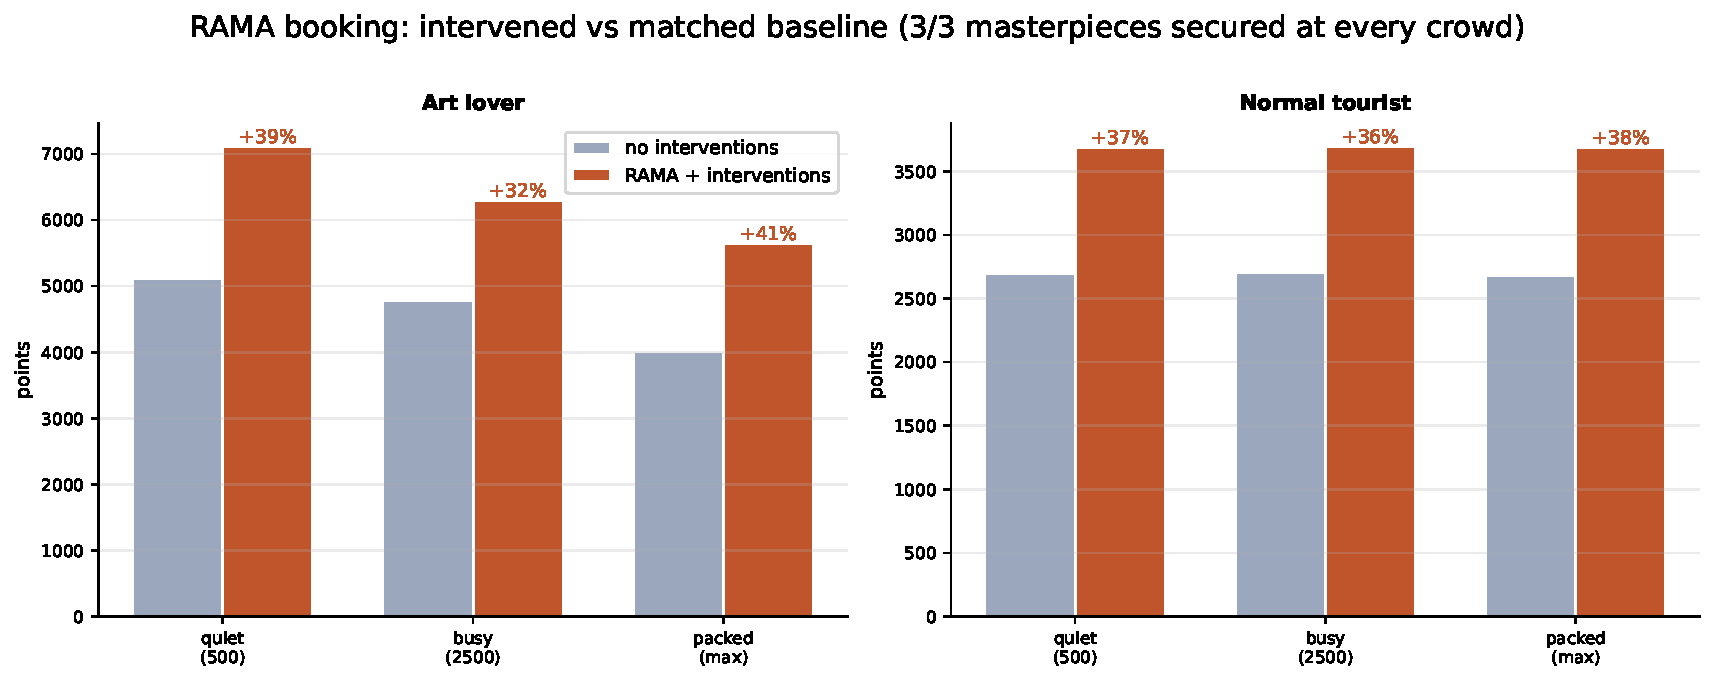
\includegraphics[width=\linewidth]{21_booking_grid.pdf}
\caption{RAMA booking gains over matched no-intervention walk baselines, reported as five-training-seed
means with standard-deviation bands.}
\label{fig:booking}
\end{figure}

\added{The high-crowd art-lover case should be read with the seed spread in mind. One favorable
trained model reaches 6,297 points at 2,500 visitors and 5,646 at 5,000 visitors under the same
six-seed deterministic evaluation. The five-reseed table is lower because it keeps the failed run
visible.} The tourist result is more stable: the shorter checklist and shorter dwell targets make it
easier to book the three windows and execute the route. The learned lead-time curve still has the
intended comparative static. Art lovers move from 7-day booking at the quiet crowd to 35-day booking
at busy and packed crowds; tourists stay at 7 days until the packed crowd, where the reseeded curve
moves later as well.

\subsection{Algorithm comparison}

Figure~\ref{fig:algorithms} shows the algorithm comparison. MaskablePPO is best or tied in every
cell. Unmasked PPO collapses for the packed tourist in the intervened world, falling to 2,093 points
where MaskablePPO reaches 3,685. DQN is competitive in several easy tourist cells but crowd-fragile for
the art lover; under the no-intervention baseline, its art-lover return falls from 4,527 at the quiet
crowd to 2,044 at the packed crowd in the five-reseed mean.

\begin{figure}[t]
\centering
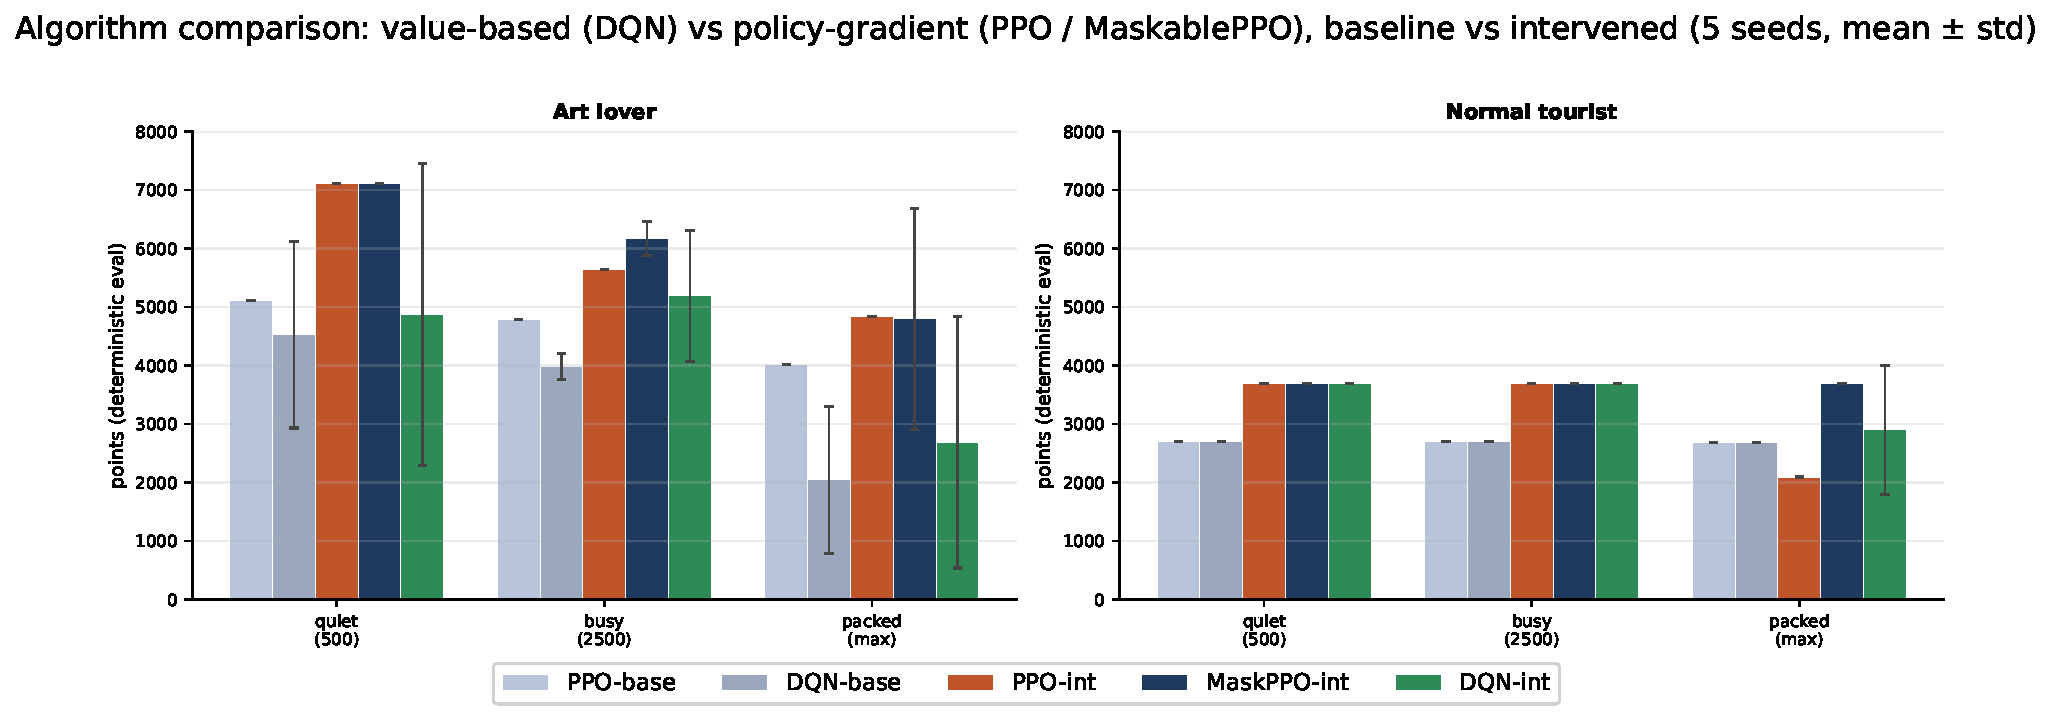
\includegraphics[width=\linewidth]{15_algorithm_comparison.pdf}
\caption{Algorithm comparison across profile and crowd cells. The dark-blue bars are MaskablePPO. The
gap to unmasked PPO at the packed tourist cell is the cleanest empirical evidence for action masking.}
\label{fig:algorithms}
\end{figure}

The pattern matches the expected weaknesses of the algorithms. DQN inherits a maximization step over
noisy value estimates, the same issue that motivates Double-Q in the tabular setting. PPO avoids that
particular max-over-actions target, but unmasked PPO still spends exploration budget discovering
actions that are impossible in the current graph or booking phase. MaskablePPO removes that burden by
matching the policy support to the legal action set at every minute.

\begin{addedblock}
\section{Failures and limitations}

The important failure modes were formulation errors, not tuning errors. The first simulator used one
guidebook tourist, which averaged away the pressure around Botticelli, Leonardo, Raphael and
Michelangelo. Splitting visitors into the 60/30/10 mix made the crowd process part of the
environment. We also had to score the visit that was still attainable at the time of booking.
Penalizing a visitor for a masterpiece slot that had already vanished made the welfare metric unfair
and gave the learner a target it could not reach.

The RL wrapper changed for the same reason. Once RAMA existed, pure route choice was no longer the
binding decision; lead time and slot timing had to become actions. A terminal no-exit penalty was too
sparse, so we added closing pressure before the deadline. Hidden dwell progress turned the same room
and clock into two different decisions, so appreciation progress entered the observation. A harsh
congestion cost made Botticelli look worse than skipping Botticelli, so crowding now discounts art
value smoothly. Booking also needed shorter credit assignment: free decline was removed, arrival
estimates were frozen, and the mismatch reward charges a bad slot near the booking step. Finally,
greedy argmax evaluation misread stochastic PPO navigation policies, so booking is evaluated
deterministically while navigation diagnostics are sampled.

These fixes are the practical lesson of the paper. The learner did not fail because PPO lacked
capacity; it failed when the MDP hid the relevant state, allowed impossible actions, delayed all
credit until the end, or optimized a reward that did not match the visitor's feasible choices.

The model is still a controlled simulation, not a live deployment estimate. Room topology and opening
hours are grounded in public sources and the official floor plan, but the 60/30/10 profile mix,
heterogeneity scale, willingness-to-pay elasticity, compliance rates and RAMA fill curve are calibrated
assumptions. The reported RAMA gain is not a pure causal estimate of RAMA alone: it compares a RAMA
policy in the all-11 world with a no-intervention walk baseline. A clean RAMA effect would need an
all-11/no-booking control. ``Always books the three masterpieces'' is a type assumption introduced
after the decline trap, not a learned preference. The RL agent is single-agent against an exogenous
crowd process, not a full multi-agent equilibrium; if many visitors used the same policy, the fill
curve and slot availability would change. The compact 8- and 25-dimensional observations also remain
partially observed approximations. Finally, welfare is a scalar proxy for art exposure, crowd comfort,
completion and timely exit; it does not settle fairness or deployment questions such as access for
visitors who cannot book early, staff operations, compliance and queue spillovers.
\end{addedblock}

\section{Conclusion}

The main lesson is that the learning problem had to be rewritten before the algorithms worked.
The status-quo visitor mostly faces a walking and dwell-time problem. The intervened
visitor faces a reservation problem with delayed payoffs, irreversible commitments and legality
constraints. Once the MDP exposes those variables, MaskablePPO learns the intended policy: reserve
masterpieces early, reserve even earlier on crowded days and pace the visit to collect the booked
windows.

At the museum level, the all-11 intervention world reduces the worst density bands and raises completed
welfare by 31\% at the 5,000-visitor crowd while preserving revenue. At the individual level, the RAMA
agent improves over optimized no-intervention baselines for both profiles and all crowds, with one
high-variance art-lover cell that is visible only when the five training reseeds are kept. The most
stable engineering takeaway is action masking: respecting the legal action set matters more than extra
tuning once the environment becomes hard.

\begin{thebibliography}{9}

\bibitem{attanasio2022}
Attanasio, A., Maravalle, M., Muccini, H., Rossi, F., Scatena, G. and Tarquini, F. (2022).
\newblock Visitors flow management at Uffizi Gallery in Florence, Italy.
\newblock \emph{Information Technology \& Tourism}, 24, 409--434.
\newblock doi:10.1007/s40558-022-00231-y.

\bibitem{centorrino2021}
Centorrino, P., et al. (2021).
\newblock Managing crowded museums: Visitors flow measurement, analysis, modeling and optimization.
\newblock \emph{Journal of Computational Science}, 53, 101357.
\newblock \added{doi:10.1016/j.jocs.2021.101357.}

\bibitem{mnih2015}
Mnih, V., et al. (2015).
\newblock Human-level control through deep reinforcement learning.
\newblock \emph{Nature}, 518, 529--533.
\newblock \added{doi:10.1038/nature14236.}

\bibitem{schulman2017}
Schulman, J., Wolski, F., Dhariwal, P., Radford, A. and Klimov, O. (2017).
\newblock Proximal policy optimization algorithms.
\newblock arXiv:1707.06347.

\bibitem{sutton2018}
Sutton, R. S. and Barto, A. G. (2018).
\newblock \emph{Reinforcement Learning: An Introduction}.
\newblock MIT Press, 2nd edition.

\bibitem{veron1989}
\added{Veron, E. and Levasseur, M. (1989).
\newblock \emph{Ethnographie de l'exposition: l'espace, le corps et le sens}.}
\newblock Bibliotheque publique d'information, Centre Georges Pompidou.

\end{thebibliography}

\end{document}
